\thispagestyle{empty}
\chapter{Vuelo Horizontal}

Las condiciones para el vuelo rectilíneo son sencillas, la velocidad vertical ha de ser nula mientras que la horizontal no. Con estas condiciones y a nivel del mar se pueden obtener las gráficas \ref{PMVH}, \ref{ControlVH}, \ref{EulerVH} y \ref{PVH}, que ofrecen una primera aproximación del rendimiento de la aeronave. De ellas se puede obtener que el valor de potencia total mínimo es de 13,354 kW, y se da para una velocidad de vuelo de 22,28 m/s. Este valor es pequeño, como cabría esperar, pero se trata de una velocidad que podría resultar útil en misiones de vigilancia por ejemplo.

\begin{figure}
	\centering
	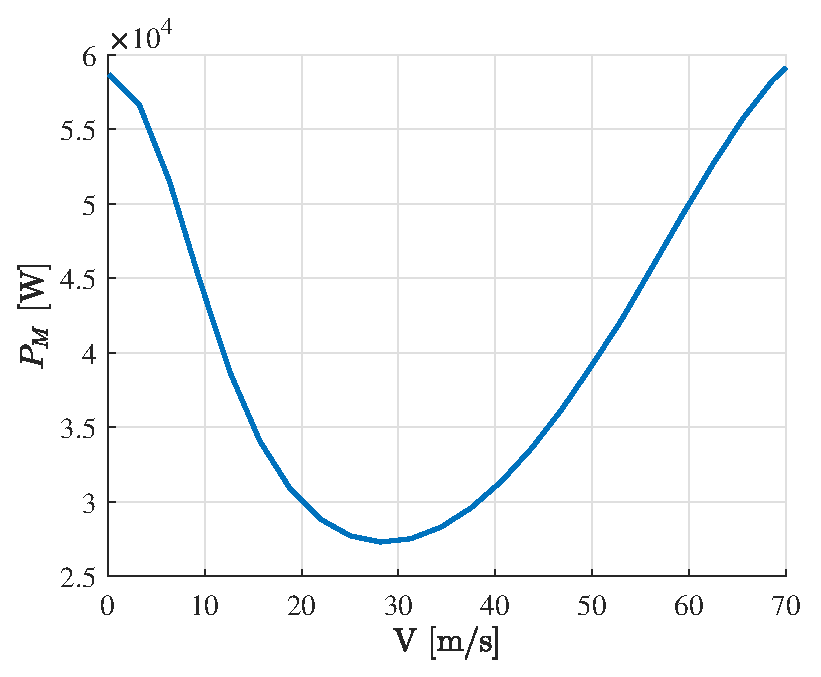
\includegraphics[width=80mm]{graficos/PMVH}
	\caption{Consumo de Potencia de la aeronave en función de la velocidad de vuelo a nivel del mar para vuelo horizontal}
	\label{PMVH}
\end{figure}
\begin{figure}
	\centering
	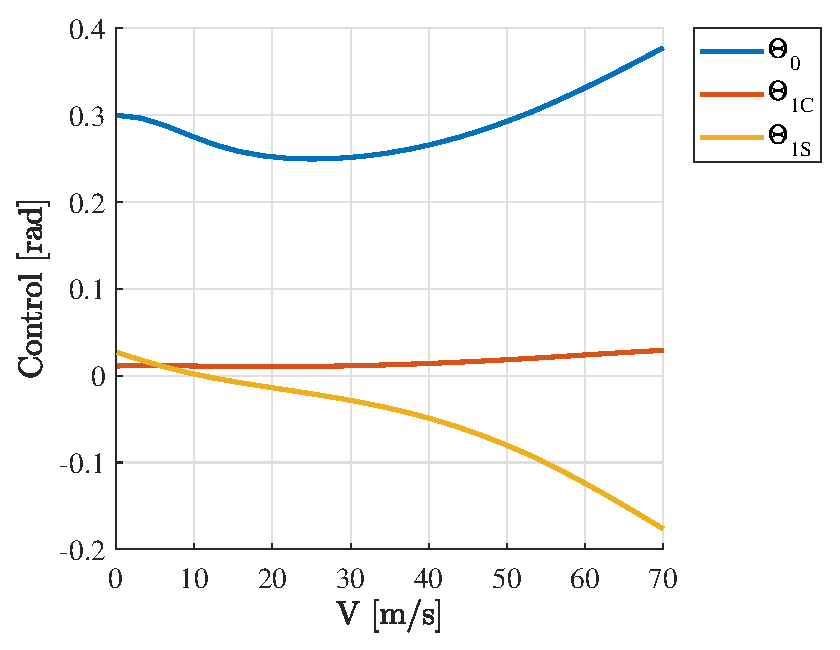
\includegraphics[width=80mm]{graficos/ControlVH}
	\caption{Ángulos de control de la aeronave en función de la velocidad de vuelo a nivel del mar para vuelo horizontal}
	\label{ControlVH}
\end{figure}
\begin{figure}
	\centering
	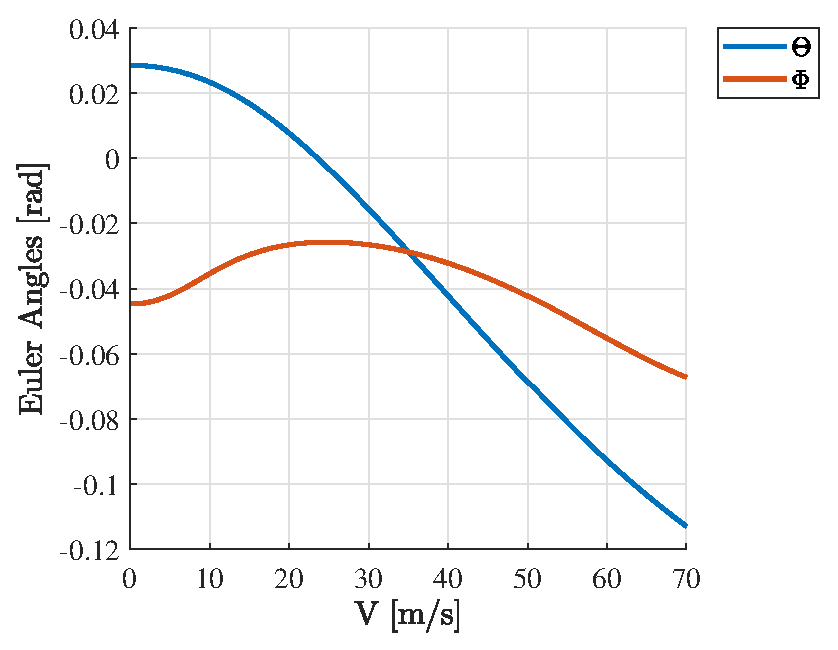
\includegraphics[width=80mm]{graficos/EulerVH}
	\caption{Ángulos de Euler de la aeronave en función de la velocidad de vuelo a nivel del mar para vuelo horizontal}
	\label{EulerVH}
\end{figure}
\begin{figure}
	\centering
	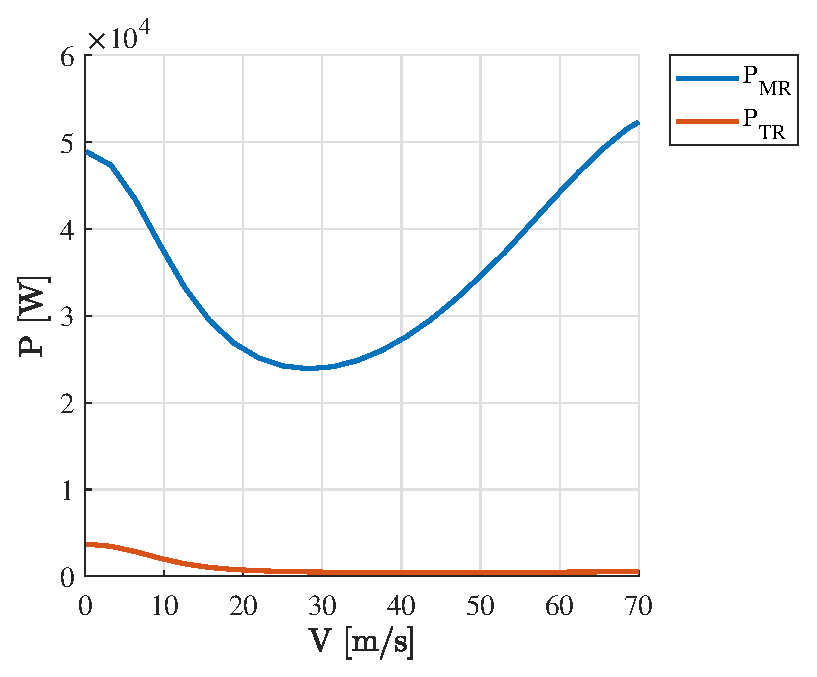
\includegraphics[width=80mm]{graficos/PVH}
	\caption{Consumo de Potencia de los rotores principal y antipar en función de la velocidad de vuelo a nivel del mar para vuelo horizontal}
	\label{PVH}
\end{figure}

Estos no son los únicos resultados útiles, 